\documentclass{standalone}
\usepackage{tikz}
\usepackage{ctex,siunitx}
\setCJKmainfont{Noto Serif CJK SC}
\usepackage{tkz-euclide}
\usepackage{amsmath}
\usetikzlibrary{patterns, calc,3d}
\usetikzlibrary {decorations.pathmorphing,decorations.pathreplacing,decorations.shapes}
\begin{document}
\small
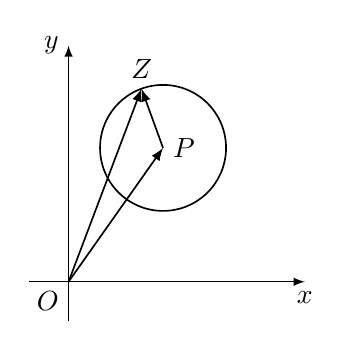
\begin{tikzpicture}[>=latex,scale=1.0]
  \draw[->](-0.5,0)--(3.0,0)node[below]{$x$};
  \draw[->](0,-0.5)--(0,3)node[left]{$y$};
  \node at (0,0)[below left]{$O$};
  \draw[semithick](1.2,1.7)circle(0.8);
  \draw[semithick,->](0,0)--(1.2,1.7)node[right]{$P$};
  \draw[semithick,->](1.2,1.7)--++(110:0.8)node[above]{$Z$};
  \draw[semithick,->](0,0)--([shift=(110:0.8)]1.2,1.7);
\end{tikzpicture}
\end{document}